\section{Entwurf}

\label{sec_impl_architecture}

In diesem Abschnitt wird basierend auf den Anforderungen aus Abschnitt \ref{sec_impl_requirements} eine von eingesetzten Verfahren unabhängige Architektur für das System entworfen. Der erste Unterabschnitt beschäftigt sich mit der Frage, an welcher Stelle in den Datenfluss zwischen Quelle der Logdaten und SIEM-System eingriffen werden kann. Anschließend wird basierend hierauf die Systemarchitektur erstellt.

\subsection{Eingriff in den Datenfluss des SIEM-Systems}

\label{sec_over_dataflow_siem}

\todo{EZ: Hier interessieren insbesondere auch die Auswirkungen auf den Rest des Systems? Wie muss das Schwellwertschema angepasst werden? Welche Akteure wissen zu welchem Zeitpunkt was? Wer bekommt welche Schluessel? Usw... Der Abschnitt hat also wesentlich mehr Potential!}

Für den Eingriff zur Pseudonymisierung der Logdaten bieten sich verschiedene Stellen im Datenfluss eines SIEM-Systems an. Im Folgenden sollen diese Möglichkeiten dargestellt und bezogen auf die in Abschnitt \ref{subsec_impl_requirements_ossimintegration} dargestellten Eigenschaften bewertet werden:
\begin{itemize}
  \item Veränderung des SIEM-Systems
  \item Nicht-pseudonymisierte Daten im SIEM-System
  \item Mehrfaches Parsen von Logdaten
  \item Abhängigkeit von Besonderheiten des SIEM-Systems
\end{itemize}
Eine Übersicht über die verschiedenen Stellen bietet Abbildung \ref{fig:siem_data_access_point}. Die Ziffern der Möglichkeiten beziehen sich auf die in der Abbildung gekennzeichneten Stellen.

\begin{figure}[]
    \centering
        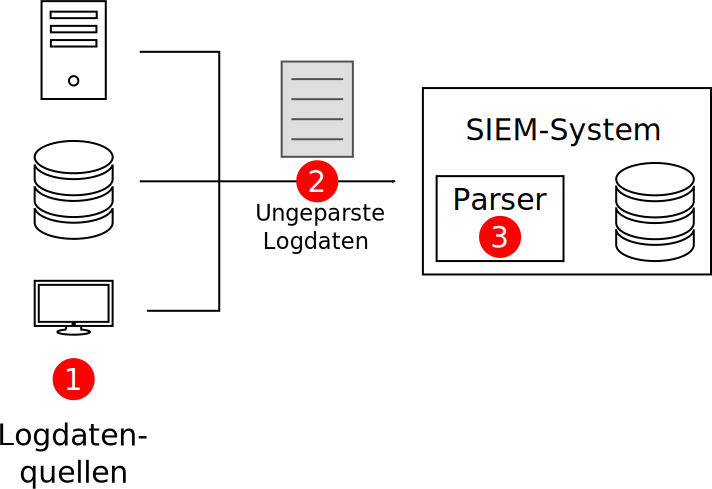
\includegraphics[width=0.5\textwidth]{dia/siem_data_access_point.pdf}
    \caption{Mögliche Eingriffspunkte in den Datenfluss eines SIEM-Systems.}
    \label{fig:siem_data_access_point}
\end{figure}

\begin{enumerate}

\item \textbf{In der Quelle der Logdaten}\\
  Bei diesem Ansatz werden die Daten bereits pseudonymisiert, bevor sie die Datenquelle verlassen. Dieser Ansatz sorgt dafür, dass die Daten bereits pseudonymisiert auf der Übertragungsstrecke und im SIEM-System vorliegen. Es ist kein mehrfaches Parsen der Daten notwendig und der Ansatz ist unabhängig vom verwendeten SIEM-System zu realisieren. Auf der anderen Seite macht der Ansatz die universelle Veränderung jeder Datenquelle notwendig. Dies kann bei Datenquellen, die auf ähnlichen gut erweiterbaren Plattformen beruhen, relativ einfach umzusetzen sein. Beispielsweise könnte die im nächsten Ansatz vorgestellte Proxy-Komponente lokal auf der Datenquelle eingesetzt werden. Schwierigkeiten würde dieser Ansatz hingegen bei Datenquellen bereithalten, die beispielsweise aus Gründen abgespeckter zugrundeliegender Betriebssysteme oder geringer Rechenleistung nur schwer erweiterbar sind. Außerdem würde er in vielen Fällen die Kooperation des Herstellers voraussetzen, wenn es sich um nicht quelloffene \glqq{}Box\grqq{}-Lösungen handelt.

\item \textbf{Proxy-basierter Ansatz}\\
  Dieser Ansatz pseudonymisiert die Daten vor dem ersten Kontakt mit dem SIEM-System, indem Datenquellen ihre Logdaten an einen Proxy senden, der die Daten pseudonymisiert und erst anschließend an das SIEM-System weiterreicht. Hierdurch wird erreicht, dass die Daten zu keiner Zeit nicht-pseudonymisiert in dem SIEM-System vorliegen. Außerdem ist er unabhängig von Datenquellen und SIEM-System und erfordert keinen direkten Eingriff in diese (abgesehen von geringen Konfigurationsanpassungen). Ein Nachteil dieser Lösung ist, dass sie das Parsen und Neuzusammensetzen der Logdaten im Proxy zusätzlich zu deren anschließender Behandlung im SIEM-System erfordert. Außerdem müssen für verschiedene Arten der Logdatenübermittlung (Protokolle wie syslog oder SNMP) unterschiedliche Proxys entwickelt werden.

\item \textbf{Patchen des SIEM-Systems}\\
  Die letzte Möglichkeit ist das Verändern des SIEM-Systems selbst. Hierzu wird in die Logdaten parsende Komponente eingegriffen, um vor, während oder nach diesem Vorgang die Logdaten zu pseudonymisieren. Dieser Ansatz erfordert kein mehrfaches Bearbeiten von Logdaten wie in dem Proxy-basierten Ansatz. Auf der anderen Seite ist er abhängig vom eingesetzten SIEM-System und erfordert seine Veränderung. Zusätzlich liegen die Daten erst einmal in nicht veränderter Form im SIEM-System vor, was die in Abschnitt \ref{subsec_impl_requirements_ossimintegration} erwähnten Nachteile mit sich bringt.

\end{enumerate}

Aus datenschutztechnischer Sicht ist eine frühestmögliche Pseudonymisierung zu bevorzugen, wie sie auch in \cite{schwartmann2017} empfohlen wird: 
\glqq{}Die Pseudonymisierung ist im Verarbeitungsprozess so früh wie möglich durchzuführen.\grqq{}
Daher wäre eine Pseudonymisierung bereits in der Datenquelle der Optimalfall. Demgegenüber stehen jedoch die erwähnten Nachteile des ersten Ansatzes im Bezug auf die Umsetzbarkeit, da hierzu jede mögliche Quelle von Logdaten universell verändert werden müsste. Eine erst im SIEM-System stattfindende Pseudonymisierung bringt jedoch die beschriebenen Risiken im Bezug auf das Vorliegen des pseudonymisierten Daten im Originalformat mit.

Dies ließ die Entscheidung auf den Proxy-basierten Ansatz fallen. Dass die Lösung außerdem noch keine Anpassungen an dem SIEM-System selbst erfordert, wiegt den Nachteil des zusätzlichen Parsens und wieder Zusammensetzens der Lognachricht bei Weitem auf.
\todo{Auch auf Angreifermodell beziehen?}

\subsection{Architektur}

%- Wie deckt dieser Ansatz die Anforderungen ab?
%  - Einbindung OSSIM
%  - Pseudonymisierung
%  - Schwellwert
%  - Benutzerinteraktion
%  - Erweiterbarkeit Datenquellen
%  - Erweiterbarkeit Datenschutztechniken

Ausgehend von diesen Überlegungen wurde ein System entworfen, dass die Anforderungen aus Abschnitt \ref{sec_impl_requirements} erfüllt und an der beschriebenen Stelle in den Datenfluss eingreift. 

%\todo{Hier erweitern: Warum verteilte Lsg (ProxyPlugin - Service):
%  - Erweiterbarkeit (Mehrere Proxy-Server mit verschiedenen Protokollen, evtl. auch direkt Client-seitig, ...) => Absicherung einer Komponente, die jedoch auch nicht alles erfährt
%  - Trennung Verarbeitung und Speicherung (Kompr. DB -> Pseudonyme bleiben verdeckt, Kompr. Proxy -> bisherige Daten und Daten evtl. anderer Proxys bleiben abgesichert)
%}

Bei dem Entwurf handelt es sich um ein verteiltes System, bei der die Verarbeitung der Logdaten und die Speicherung der Pseudonymzuordnung an unterschiedlichen Stellen geschieht. Hierfür sprechen verschiedene Gründe. Die Kompromittierung der speichernden Komponente schützt die erstellten Pseudonyme vor Aufdeckung durch die Verschlüsselung der Datensätze mit einem kryptographischen Schwellwertschema. Die Kompromittierung der verarbeitenden Komponente lässt zwar eine Verknüpfung neu erstellter Pseudonyme mit eintreffenden Daten zu, sorgt aber nicht für eine Aufdeckung bereits erstellter Pseudonyme, da diese in der anderen Komponente vorliegen. Weiterhin sorgt dieser Ansatz auch für eine zusätzliche Erweiterbarkeit des Systems. Eine speichernde Komponente kann so als Datenspeicher für mehrere verarbeitende Komponenten agieren, was beispielsweise die Erweiterung um zusätzliche Protokolle (vgl. Abschnitt \ref{sec_impl_integration_into_ossim}) oder Pseudonyme über verschiedene Datenarten (vgl. Abschnitt \ref{sec_state_se_furtherpossibilities}) ermöglicht.
Einen Überblick über den Entwurf bietet Abbildung \ref{fig:high__level_architecture}. Die verschiedenen Komponenten des Systems werden im Folgenden näher beschrieben.

\begin{figure}[]
    \centering
        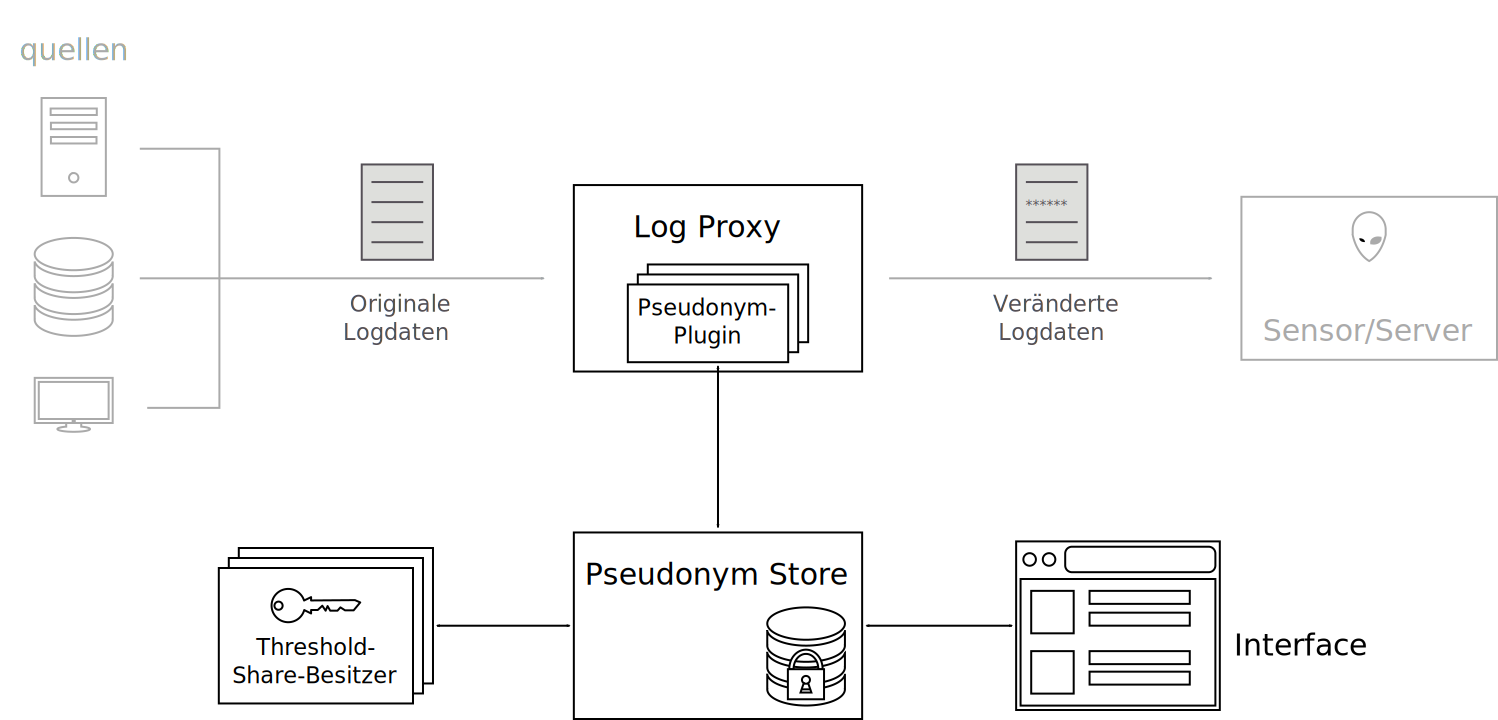
\includegraphics[width=0.9\textwidth]{dia/high_level_architecture.pdf}
    \caption{Ein Überblick über die entworfene Architektur.}
    \label{fig:high__level_architecture}
\end{figure}

Die erste Komponente ist der \textbf{Log-Proxy}, der die Daten entgegennimmt, verändert und anschließend an das SIEM-System weiterleitet. Das Verändern der Daten kann mit verschiedenen Plugins geschehen, so dass neben der umzusetzenden Pseudonymisierung auch weitere Datenschutztechniken eingesetzt werden können, was die geforderte Erweiterbarkeit aus Abschnitt \ref{subsec_impl_requirements_plugins} ermöglicht. Der Proxy leistet die Behandlung von Logdaten aus verschiedenen Quellen wie in Abschnitt \ref{subsec_impl_requirements_differentsources} beschrieben. Das für diese Art des Dateneingriffs erforderliche Parsen und Wiederzusammensetzen der Daten muss hier Datenquellen-abhängig konfigurierbar geschehen.

Ein in dem Proxy enhaltenes Plugin ist für die Pseudonymisierung von Daten zuständig und kommuniziert dazu mit einer externen Komponente -- dem Pseudonym-Service. Die Kommunikation mit dem Proxy erfolgt über einen Webservice-basierten Ansatz. Das Plugin kann für eingehende Daten ein Pseudonym anfordern und dieses anschließend in der Logdatenverarbeitung verwenden.

Der \textbf{Pseudonym-Service} erfüllt zwei Aufgaben: das Speichern und Verwalten der Pseudonyme sowie die Integrierung des kryptographischen Schwellwertschemas. Initial muss die Schlüsselgenerierung des Schwellwertschemas durch den Service geleistet werden. Dies kann wie bereits im vorhergehenden Abschnitt beschrieben zentral oder verteilt geschehen.\\
Es können während des Betriebs neue Pseudonyme angelegt und zusammen mit ihrem durch das Schwellwertschema verschlüsselten Datum abgelegt werden. Sie werden durch geeignete Maßnahmen durchsuchbar gehalten, um für ein Datum überprüfen zu können, ob bereits ein Pseudonym vergeben wurde. 
Über ein Webinterface kann ein berechtiger Benutzer die Aufdeckung eines bestimmten Pseudonyms fordern und den Status seiner Forderung bzw. im Erfolgsfall das aufgedeckte Datum betrachten. Dieses Datum wird durch das Kombinieren der partiellen Entschlüsselungen erhalten, die von den entsprechenden \textit{Share}-Besitzern berechnet werden. Weiterhin kann über dieses Webinterface auch die initiale Konfiguration des Systems im Bezug auf Eigenschaften des Pseudonymisierung und des kryptographischen Schwellwertschemas vorgenommen werden.

Benutzer, die zuständig für die Bewertung von Anfragen zur Aufdeckung eines Pseudonyms sind, erhalten die Möglichkeit zur Interaktion mit dem System über eine \textbf{Client-Anwendung}, für die der Pseudonym-Service ebenfalls als Webservice agiert. Diese Anwendung verwaltet den \textit{Share} des Benutzers für das kryptographische Schwellwertschema und kann nach der Bestätigung des Benutzers zu der Aufdeckung eines Pseudonyms die partielle Entschlüsselung eines Datensatzes erstellen und an den Pseudonym-Service senden.
